% =============================================================
%  UNIG conceptual diagram — TikZ source (vector)
%  Compile standalone:  pdflatex unig_overview_tikz.tex
%  Produces unig_overview_tikz.pdf; rename/copy to fig/unig_overview.pdf
%  or \input this file inside a figure environment (requires tikz).
% =============================================================
\documentclass[border=4pt]{standalone}
\usepackage{tikz}
\usetikzlibrary{positioning}
\usepackage{helvet}
\renewcommand{\familydefault}{\sfdefault}

% ---- palette ------------------------------------------------
\definecolor{unigblue}{RGB}{0,120,220}    % Phase 1
\definecolor{unigyellow}{RGB}{190,150,0}  % Phase 2
\definecolor{unigtan}{RGB}{168,134,86}    % generation
\definecolor{unigslate}{RGB}{96,115,136}  % data center load
\definecolor{unigtext}{RGB}{40,40,40}

\begin{document}
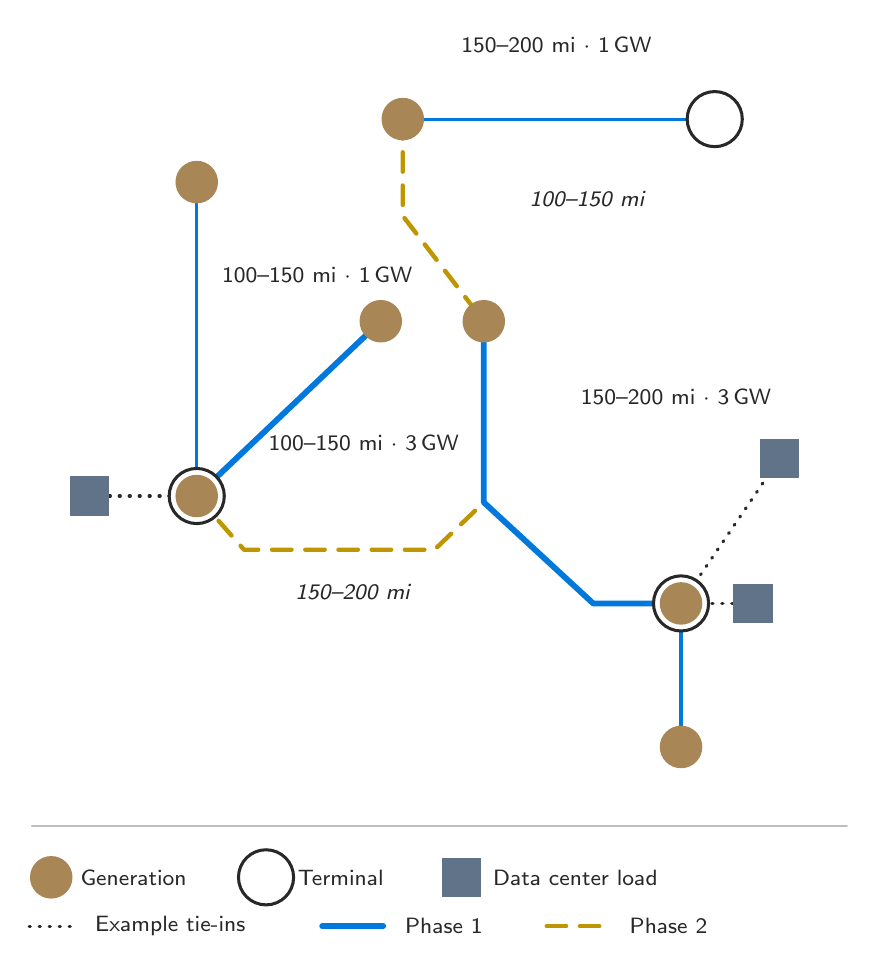
\begin{tikzpicture}[
    scale=0.62,
    every node/.style={transform shape=false},
    line cap=round, line join=round,
    link1/.style={unigblue, line width=1.15pt},          % 1 GW link
    link3/.style={unigblue, line width=2.10pt},          % 3 GW link
    phase2/.style={unigyellow, line width=1.60pt, dash pattern=on 7pt off 5pt},
    tiein/.style={unigtext, line width=1.15pt, dash pattern=on 0.4pt off 3.2pt},
    gen/.style={circle, fill=unigtan, inner sep=0pt, minimum size=5.4mm},
    term/.style={circle, draw=unigtext, line width=1.1pt, fill=white,
                 inner sep=0pt, minimum size=7.0mm},
    load/.style={rectangle, fill=unigslate, inner sep=0pt, minimum size=5.0mm},
    lbl/.style={unigtext, font=\footnotesize},
    lblit/.style={unigtext, font=\footnotesize\itshape},
  ]

  % ---- node coordinates (from the UNIG conceptual layout) ----
  \coordinate (G1)    at ( 7.95,14.78);   % north generation
  \coordinate (TN)    at (14.34,14.78);   % north terminal
  \coordinate (G2)    at ( 3.73,13.49);   % north-west generation
  \coordinate (G3)    at ( 7.50,10.64);   % central-west generation
  \coordinate (G4)    at ( 9.61,10.64);   % central generation
  \coordinate (TW)    at ( 3.73, 7.06);   % west terminal
  \coordinate (J)     at ( 9.61, 6.93);   % central junction
  \coordinate (BEND)  at (11.85, 4.86);   % bend towards south-east terminal
  \coordinate (TSE)   at (13.65, 4.86);   % south-east terminal
  \coordinate (G7)    at (13.65, 1.92);   % south generation
  \coordinate (L1)    at (15.67, 7.83);   % load, north-east
  \coordinate (L2)    at ( 1.53, 7.06);   % load, west
  \coordinate (L3)    at (15.12, 4.86);   % load, south-east

  % ---- Phase 1 links ----------------------------------------
  \draw[link1] (G1)  -- (TN);
  \draw[link1] (G2)  -- (TW);
  \draw[link3] (G3)  -- (TW);
  \draw[link3] (G4)  -- (J) -- (BEND) -- (TSE);
  \draw[link1] (TSE) -- (G7);

  % ---- Phase 2 links ----------------------------------------
  \draw[phase2] (G1) -- ( 7.95,12.80) -- (G4);
  \draw[phase2] (TW) -- ( 4.70, 5.96) -- ( 8.60, 5.96) -- (J);

  % ---- example tie-ins --------------------------------------
  \draw[tiein] (L2)  -- (TW);
  \draw[tiein] (L1)  -- (TSE);
  \draw[tiein] (L3)  -- (TSE);

  % ---- markers ----------------------------------------------
  \node[gen]  at (G1) {};
  \node[gen]  at (G2) {};
  \node[gen]  at (G3) {};
  \node[gen]  at (G4) {};
  \node[gen]  at (G7) {};
  \node[load] at (L1) {};
  \node[load] at (L2) {};
  \node[load] at (L3) {};
  \node[term] at (TN) {};
  \node[term] at (TW) {}; \node[gen] at (TW) {};
  \node[term] at (TSE){}; \node[gen] at (TSE){};

  % ---- labels -----------------------------------------------
  \node[lbl,   anchor=south]      at (11.10,15.95) {150--200 mi $\cdot$ 1\,GW};
  \node[lblit, anchor=west]       at (10.35,13.15) {100--150 mi};
  \node[lbl,   anchor=west]       at ( 4.05,11.60) {100--150 mi $\cdot$ 1\,GW};
  \node[lbl,   anchor=east]       at ( 9.30, 8.15) {100--150 mi $\cdot$ 3\,GW};
  \node[lbl,   anchor=west]       at (11.40, 9.10) {150--200 mi $\cdot$ 3\,GW};
  \node[lblit, anchor=west]       at ( 5.55, 5.10) {150--200 mi};

  % ---- legend -----------------------------------------------
  \draw[unigtext!30, line width=0.6pt] (0.35,0.30) -- (17.05,0.30);

  \node[gen]  at (0.75,-0.75) {};
  \node[lbl, anchor=west] at (1.15,-0.75) {Generation};
  \node[term] at (5.15,-0.75) {};
  \node[lbl, anchor=west] at (5.60,-0.75) {Terminal};
  \node[load] at (9.15,-0.75) {};
  \node[lbl, anchor=west] at (9.60,-0.75) {Data center load};

  \draw[tiein]  (0.30,-1.75) -- (1.20,-1.75);
  \node[lbl, anchor=west] at (1.45,-1.75) {Example tie-ins};
  \draw[link3]  (6.30,-1.75) -- (7.55,-1.75);
  \node[lbl, anchor=west] at (7.80,-1.75) {Phase 1};
  \draw[phase2] (10.90,-1.75) -- (12.15,-1.75);
  \node[lbl, anchor=west] at (12.40,-1.75) {Phase 2};

\end{tikzpicture}
\end{document}
